\let\negmedspace\undefined
\let\negthickspace\undefined
\documentclass[journal]{IEEEtran}
\usepackage[a5paper, margin=10mm, onecolumn]{geometry}
\usepackage{lmodern} % Ensure lmodern is loaded for pdflatex
\usepackage{tfrupee} % Include tfrupee package

\setlength{\headheight}{1cm} % Set the height of the header box
\setlength{\headsep}{0mm}     % Set the distance between the header box and the top of the text

\usepackage{gvv-book}
\usepackage{gvv}
\usepackage{cite}
\usepackage{amsmath,amssymb,amsfonts,amsthm}
\usepackage{algorithmic}
\usepackage{graphicx}
\usepackage{textcomp}
\usepackage{xcolor}
\usepackage{txfonts}
\usepackage{listings}
\usepackage{enumitem}
\usepackage{mathtools}
\usepackage{gensymb}
\usepackage{comment}
\usepackage[breaklinks=true]{hyperref}
\usepackage{tkz-euclide} 
\usepackage{listings}
\usepackage{gvv}                                        
\def\inputGnumericTable{}                                 
\usepackage[latin1]{inputenc}                                
\usepackage{color}                                            
\usepackage{array}                                            
\usepackage{longtable}                                       
\usepackage{calc}                                             
\usepackage{multirow}                                         
\usepackage{hhline}                                           
\usepackage{ifthen}                                           
\usepackage{lscape}

\begin{document}
\bibliographystyle{IEEEtran}
\begin{center}
    \textbf{\Large GATE(2023)}
    
    \textbf{Aerospace Engineering (AE)}
    \end{center}

\textbf{\Large Q.1 - Q.5 carry one mark each.}

\begin{enumerate}
\item A student is required to demonstrate a high level of \textit{comprehension} of the subject, especially in the social sciences.

The word closest in meaning to \textit{comprehension} is

\begin{enumerate}
    \item understanding
    \item meaning
    \item concentration
    \item stability
\end{enumerate}
\hfill{\brak{\text{GATE AE 2014}}}


\item  Choose the most appropriate word from the options given below to complete the following sentence.

One of his biggest \underline{\hspace{1cm}} was his ability to forgive.

\begin{enumerate}
    \item vice
    \item virtues
    \item choices
    \item strength
\end{enumerate}
\hfill{\brak{\text{GATE AE 2014}}}


\item Rajan was not happy that Sajan decided to do the project on his own. On observing his unhappiness, Sajan explained to Rajan that he preferred to work independently.


Which one of the statements below is logically valid and can be inferred from the above sentences?

\begin{enumerate}
    \item Rajan has decided to work only in a group.
    \item Rajan and Sajan were formed into a group against their wishes.
    \item Sajan had decided to give in to Rajan's request to work with him.
    \item Rajan had believed that Sajan and he would be working together.
\end{enumerate}
\hfill{\brak{\text{GATE AE 2014}}}

\item If $y = 5x^{2} + 3$, then the tangent at $x = 0, y = 3$

\begin{enumerate}
    \item passes through $x = 0, y = 0$
    \item has a slope of $+1$
    \item is parallel to the $x$-axis
    \item has a slope of $-1$
\end{enumerate}
\hfill{\brak{\text{GATE AE 2014}}}
\newpage
\item A foundry has a fixed daily cost of Rs 50,000 whenever it operates and a variable cost of Rs $800Q$, where $Q$ is the daily production in tonnes. What is the cost of production in Rs per tonne for a daily production of 100 tonnes?
\begin{figure}[H]
    \centering
    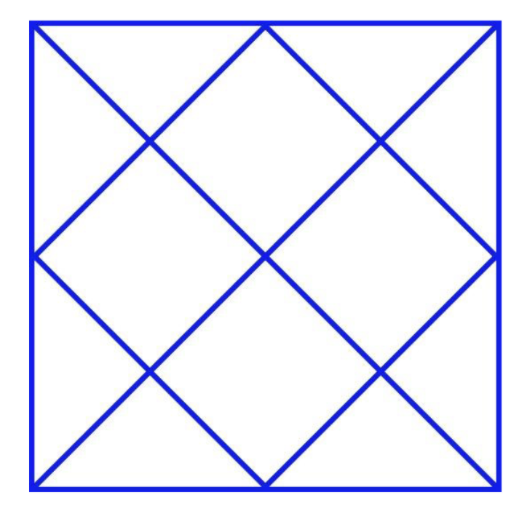
\includegraphics[width=0.5\columnwidth]{Figs/Q5.png}
    \caption{}
    \label{fig:placeholder}
\end{figure}

\textbf{\Large Q.6 - Q.10carry two mark each.}

\item Find the odd one in the following group:
\[
\texttt{ALRVX},\ \texttt{EPVZB},\ \texttt{ITZDF},\ \texttt{OYEIK}
\]

\medskip

\begin{enumerate}
  \item \texttt{ALRVX}
  \item \texttt{EPVZB}
  \item \texttt{ITZDF}
  \item \texttt{OYEIK}
\end{enumerate}
\hfill{\brak{\text{GATE AE 2014}}}

\item Anuj, Bhola, Chandan, Dilip, Eswar and Faisal live on different floors in a six-storeyed building (the ground floor is numbered 1, the floor above it 2, and so on). Anuj lives on an even-numbered floor. Bhola does not live on an odd numbered floor. Chandan does not live on any of the floors below Faisal's floor. Dilip does not live on floor number 2. Eswar does not live on a floor immediately above or immediately below Bhola. Faisal lives three floors above Dilip. Which of the following floor-person combinations is correct?


\begin{center}
\begin{tabular}{|c|c|c|c|c|c|c|}
\hline
 & Anuj & Bhola & Chandan & Dilip & Eswar & Faisal \\
\hline
(A) & 6 & 2 & 5 & 1 & 3 & 4 \\
\hline
(B) & 2 & 6 & 5 & 1 & 3 & 4 \\
\hline
(C) & 4 & 2 & 6 & 3 & 1 & 5 \\
\hline
(D) & 2 & 4 & 6 & 1 & 3 & 5 \\
\hline
\end{tabular}
\end{center}
\hfill{\brak{\text{GATE AE 2014}}}

\item The smallest angle of a triangle is equal to two thirds of the smallest angle of a quadrilateral. The ratio between the angles of the quadrilateral is $3 : 4 : 5 : 6$. The largest angle of the triangle is twice its smallest angle. What is the sum, in degrees, of the second largest angle of the triangle and the largest angle of the quadrilateral?

\hfill{\brak{\text{GATE AE 2014}}}


\item One percent of the people of country X are taller than 6 ft. Two percent of the people of country Y are taller than 6 ft. There are thrice as many people in country X as in country Y. Taking both countries together, what is the percentage of people taller than 6 ft?


\begin{enumerate}
    \item 3.0
    \item 2.5
    \item 1.5
    \item 1.25
\end{enumerate}
\hfill{\brak{\text{GATE AE 2014}}}

\item The monthly rainfall chart based on 50 years of rainfall in Agra is shown in the following figure. Which of the following are true? (\(k\) percentile is the value such that \(k\) percent of the data fall below that value)

\begin{figure}[H]
\centering
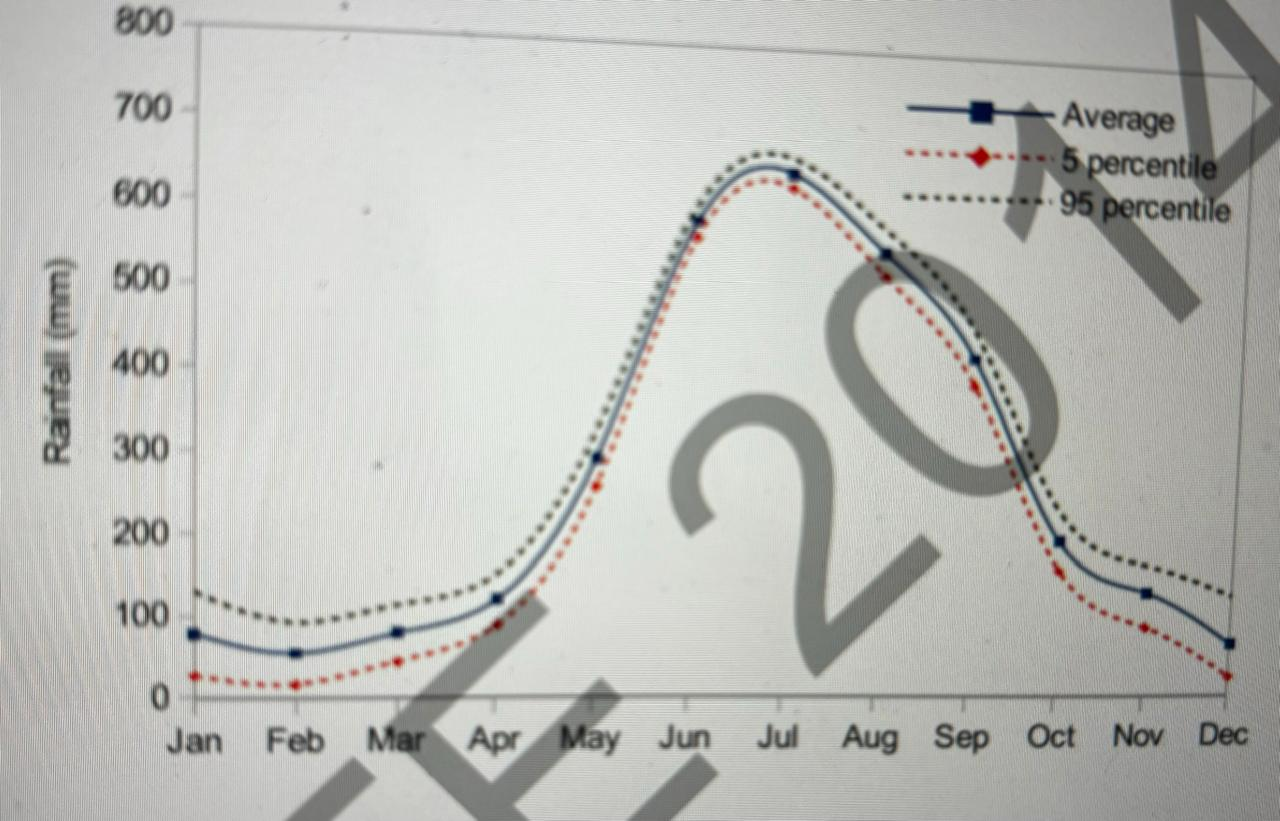
\includegraphics[width=0.5\columnwidth]{Figs/TT.jpeg}
\caption{}
\end{figure}

    \begin{enumerate}
        
    \item On average, it rains more in July than in December
    \item Every year, the amount of rainfall in August is more than that in January
    \item July rainfall can be estimated with better confidence than February rainfall
    \item In August, there is at least 500 mm of rainfall
\end{enumerate}


\begin{enumerate}
    \item (i) and (ii)
    \item (i) and (iii)
    \item (ii) and (iii)
    \item (iii) and (iv)
    
\end{enumerate}

\hfill{\brak{\text{GATE AE 2014}}}

\section*{Q.1 -- Q.25 carry one mark each}

\item For a real symmetric matrix \([A]\), which of the following statements is true?

\begin{enumerate}
    \item The matrix is always diagonalizable and invertible.
    \item The matrix is always invertible but not necessarily diagonalizable.
    \item The matrix is always diagonalizable but not necessarily invertible.
    \item The matrix is always neither diagonalizable nor invertible.
\end{enumerate}
\hfill{\brak{\text{GATE AE 2014}}}

\item The series 
\[
s = \sum_{m=1}^{\infty} \frac{m^{2}}{3^{m}} (x - 2)^{m}
\]
converges for all \(x\) with \(|x - 2| \le R\) given by

\begin{enumerate}
    \item \(R = 0\)
    \item \(R = 3\)
    \item \(R = \infty\)
    \item \(R = \frac{1}{3}\)
\end{enumerate}
\hfill{\brak{\text{GATE AE 2014}}}

\item The function given by
\[
f(x) =
\begin{cases}
\sin\left(\frac{1}{x}\right), & x \neq 0 \\
0, & x = 0
\end{cases}
\]
is

\begin{enumerate}
    \item Unbounded everywhere
    \item Bounded and continuous everywhere
    \item Bounded but not continuous at \(x = 0\)
    \item Continuous and differentiable everywhere
\end{enumerate}
\hfill{\brak{\text{GATE AE 2014}}}

\item Given the boundary-value problem
\[
\frac{d}{dx} \left( \frac{dy}{dx} \right) + k y = 0,\quad 0 < x < 1,\quad \text{with } y(0) = y(1) = 0.
\]
Then the solutions of the boundary-value problem for \( k = 1 \) (given by \( y_1 \)) and \( k = 5 \) (given by \( y_5 \)) satisfy:

\begin{enumerate}
    \item \(\displaystyle \int_0^1 y_1 y_5 \, dx = 0\)
    \item \(\displaystyle \int_0^1 \frac{dy_1}{dx} \frac{dy_5}{dx} \, dx = 0\)
    \item \(\displaystyle \int_0^1 y_1 y_5 \, dx \ne 0\)
    \item \(\displaystyle \int_0^1 \left( y_1 y_5 + \frac{dy_1}{dx} \frac{dy_5}{dx} \right) dx = 0\)
\end{enumerate}
\hfill{\brak{\text{GATE AE 2014}}}

\item The value of
\[
I = \int_{0}^{1} 1000x^{4} \, dx
\]
obtained by using Simpson's rule with 2 equally spaced intervals is,

\begin{enumerate}
    \item 200
    \item 400
    \item 180
    \item 208
\end{enumerate}
\hfill{\brak{\text{GATE AE 2014}}}

\item For a \textit{NACA} 5-digit airfoil of chord $c$, the designed lift coefficient and location of maximum camber along the chord from the leading edge are denoted by $C_L$ and $X_m$ respectively. For \textit{NACA12018} airfoil, which combination of $C_L$ and $X_m$ given below are correct?

\begin{enumerate}
    \item $C_L = 0.15$ and $X_m = 0.1c$
    \item $C_L = 0.12$ and $X_m = 0.2c$
    \item $C_L = 0.12$ and $X_m = 0.18c$
    \item $C_L = 0.15$ and $X_m = 0.2c$
\end{enumerate}
\hfill{\brak{\text{GATE AE 2014}}}

\item For inviscid, supersonic flow over a diamond shaped airfoil, shown in the figure, which statement is correct among the following?

\begin{figure}[H]
\centering
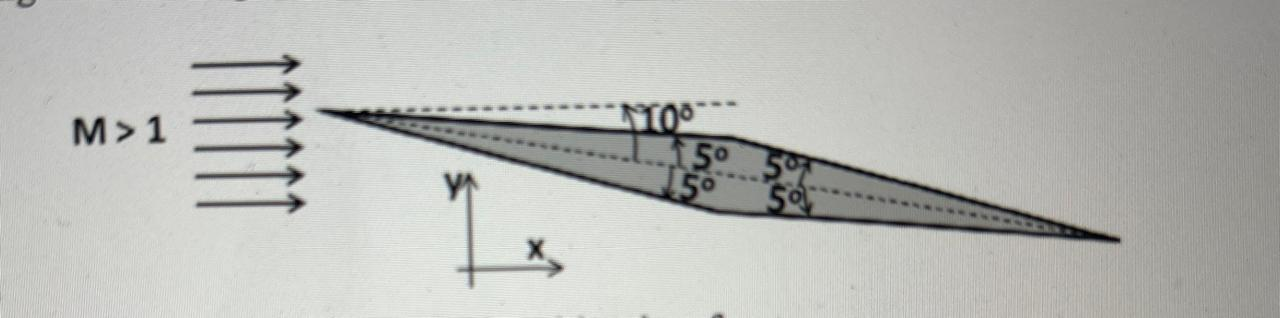
\includegraphics[width=0.5\columnwidth]{Figs/pp.jpeg}
\caption{}
\end{figure}


\begin{enumerate}
    \item The airfoil will experience zero lift and positive drag force
    \item The airfoil will experience positive lift and zero drag force
    \item The airfoil will experience negative lift and zero drag force
    \item The airfoil will experience positive lift and positive drag force
\end{enumerate}
\hfill{\brak{\text{GATE AE 2014}}}

\item Consider supersonic flow near a corner (at an angle $\theta$ from the horizontal) with an attached oblique shock (at an angle $\beta$ with horizontal) as shown in figure. If Mach number $M$ decreases gradually from a high supersonic value, which of the following statements is correct?
\begin{figure}[H]
\centering
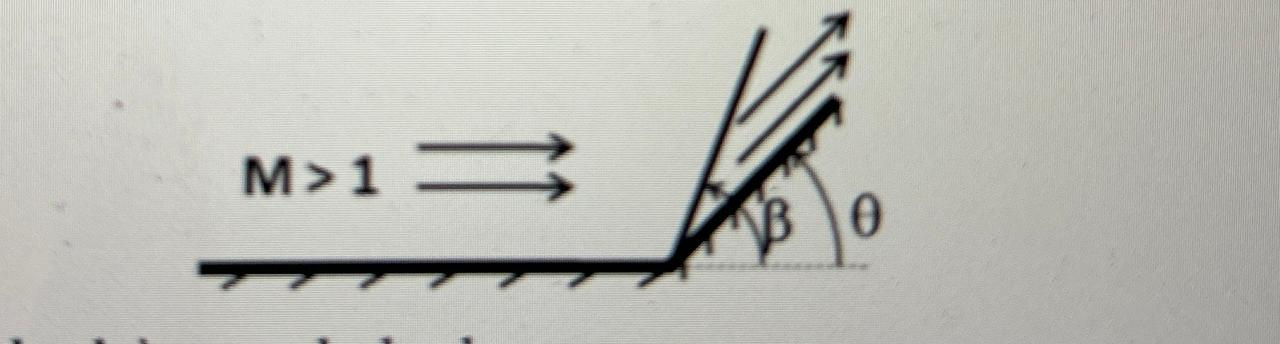
\includegraphics[width=0.5\columnwidth]{Figs/mm.jpeg}
\caption{}
\end{figure}

\begin{enumerate}
    \item $\beta$ will decrease if the shock is a weak shock
    \item $\beta$ will decrease if the shock is a strong shock
    \item $\beta$ will increase for both weak and strong shocks
    \item $\beta$ remains unchanged for both weak and strong shocks
\end{enumerate}
\hfill{\brak{\text{GATE AE 2014}}}

\item The streamlines of a potential line vortex is concentric circles with respect to the vortex center as shown in figure. Velocity along these streamlines, outside the core of the vortex can be written as,
$$
v_{\theta} = \frac{\Gamma}{2 \pi r},
$$
where strength of the vortex is $\Gamma$ and $r$ is radial direction. The value of circulation along the curve shown in the figure is:

\begin{figure}[H]
\centering
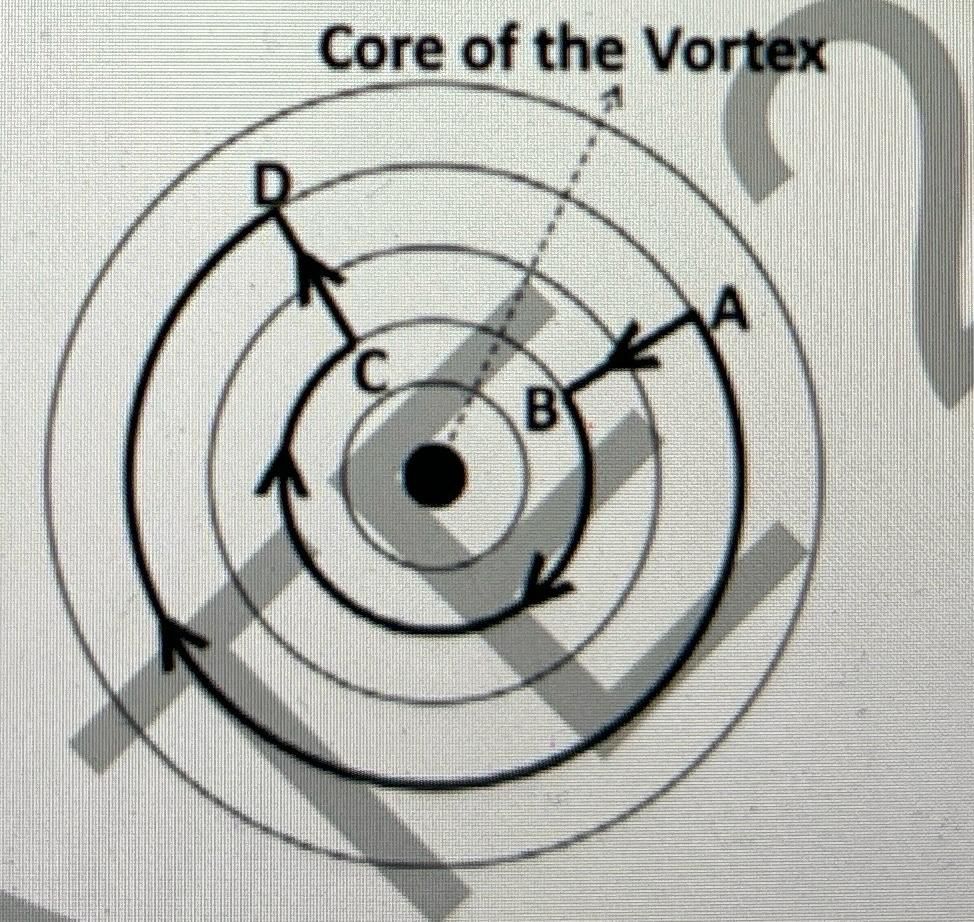
\includegraphics[width=0.4\columnwidth]{Figs/oo.jpeg}
\caption{}
\end{figure}
\begin{enumerate}
    \item $\Gamma$
    \item $-2\Gamma$
    \item $2\Gamma$
    \item $0$
\end{enumerate}
\hfill{\brak{\text{GATE AE 2014}}}

\item To observe unsteady separated flow in a diverging channel, bubbles are injected at each $10\,\mathrm{ms}$ interval at point A as shown in figure. These bubbles act as tracer particles and follow the flow faithfully. The curved line AB shown at any instant represents:
\begin{figure}[H]
\centering
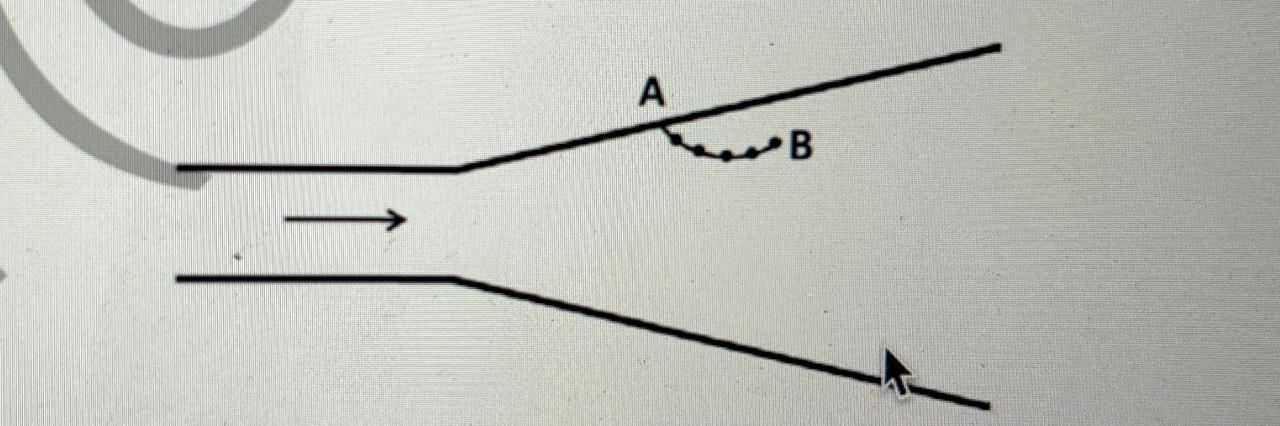
\includegraphics[width=0.4\columnwidth]{Figs/cc.jpeg}
\caption{}
\end{figure}
\begin{enumerate}
    \item Streamline, streakline and pathline
    \item Streamline and pathline
    \item Only a pathline
    \item Only a streakline
\end{enumerate}
\hfill{\brak{\text{GATE AE 2014}}}

\item It is desired to measure the Young's modulus and the Poisson's ratio of a given homogeneous, isotropic material. A bar of length $20\,\mathrm{cm}$ and square cross-section ($10\,\mathrm{mm} \times 10\,\mathrm{mm}$) of this material is subjected to a tensile load of $40\,\mathrm{kN}$. Under this load, length increases to $20.1\,\mathrm{cm}$ while the cross-section reduces to $9.98\,\mathrm{mm} \times 9.98\,\mathrm{mm}$. Young's modulus and Poisson's ratio of the material are:

\begin{enumerate}
    \item $80\,\mathrm{GPa} \ \& \ 0.4$ respectively
    \item $40\,\mathrm{GPa} \ \& \ -0.4$ respectively
    \item $80\,\mathrm{GPa} \ \& \ -0.2$ respectively
    \item $40\,\mathrm{GPa} \ \& \ 0.2$ respectively
\end{enumerate}
\hfill{\brak{\text{GATE AE 2014}}}

\item In general, for any given solid subjected to arbitrary loading, which of the following statements is \textit{always} true:

\begin{enumerate}
    \item Volume does not vary with loading
    \item Mass does not vary with loading
    \item Density does not vary with loading
    \item Volume, mass and density vary with loading
\end{enumerate}
\hfill{\brak{\text{GATE AE 2014}}}

\item Which one of the following objects with inclined face at $45^\circ$, subjected to the given stresses, are in static equilibrium:
\begin{figure}[H]
\centering
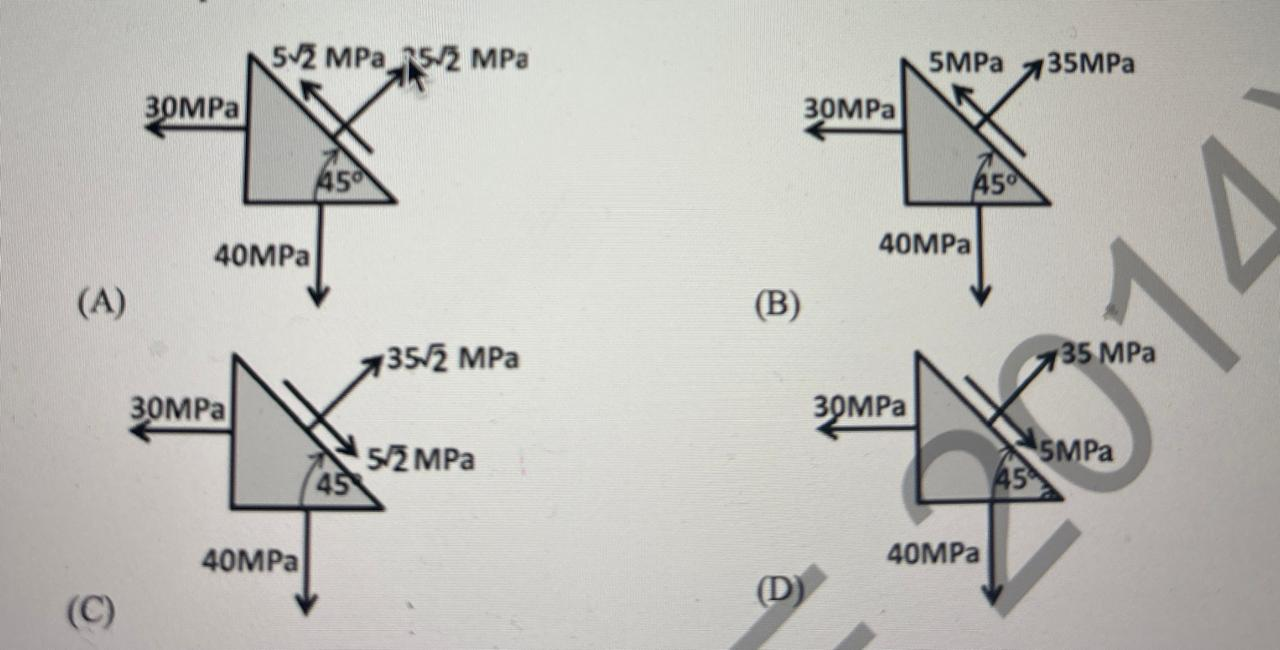
\includegraphics[width=0.8\columnwidth]{Figs/q13.jpeg}
\caption{}
\end{figure}
\hfill{\brak{\text{GATE AE 2014}}}

\item  
A damped single degree of freedom system whose undamped natural frequency, $\omega_n = 10$ Hz, is subjected to sinusoidal external force.  
Power is half of the maximum for the two frequencies of $60.9469$ rad/s and $64.168$ rad/s.  
The damping factor associated with the vibrating system (in \%) is:

\item  
The boundary conditions for a rod with circular cross-section, under torsional vibration, are changed from fixed-free to fixed-fixed.  
The fundamental natural frequency of the fixed-fixed rod is $k$ times that of fixed-free rod.  
The value of $k$ is:

\begin{enumerate}
    \item 1.5
    \item $\pi$
    \item 2.0
    \item 0.5
\end{enumerate}
\hfill{\brak{\text{GATE AE 2014}}}

\item  
Match the appropriate engine (in right column) with the corresponding aircraft (in left column)  
for most efficient performance of the engine.

\begin{multicols}{2}
\textbf{Left column:}
\begin{enumerate}
    \item Low speed transport aircraft
    \item High subsonic civilian aircraft
    \item Supersonic fighter aircraft
    \item Hypersonic aircraft
\end{enumerate}

\columnbreak
\textbf{Right column:}
\begin{enumerate}
    \item Ramjet
    \item Turboprop
    \item Turbojet
    \item Turbofan
\end{enumerate}
\end{multicols}

\begin{enumerate}
    \item a -- iv, b -- iii, c -- i, d -- ii
    \item a -- ii, b -- i, c -- iii, d -- iv
    \item a -- i, b -- ii, c -- iv, d -- iii
    \item a -- ii, b -- iv, c -- iii, d -- i
\end{enumerate}
\hfill{\brak{\text{GATE AE 2014}}}

\item  
For a given fuel flow rate and thermal efficiency, the take-off thrust for a gas turbine engine  
burning aviation turbine fuel (considering fuel-air ratio $f \ll 1$) is  

\begin{enumerate}
    \item Directly proportional to exhaust velocity
    \item Inversely proportional to exhaust velocity
    \item Independent of exhaust velocity
    \item Directly proportional to the square of the exhaust velocity
\end{enumerate}
\hfill{\brak{\text{GATE AE 2014}}}

\item  
For a fifty percent reaction axial compressor stage, following statements are given:  
I. Velocity triangles at the entry and exit of the rotor are symmetrical  
II. The whirl or swirl component of absolute velocity at the entry of rotor and entry of stator are same.  

Which of the following options are correct?  
\begin{enumerate}
    \item Both I and II are correct statements
    \item I is correct but II is incorrect
    \item I is incorrect but II is correct
    \item Both I and II are incorrect
\end{enumerate}
\hfill{\brak{\text{GATE AE 2014}}}

\item  
A small rocket having a specific impulse of $200\,s$ produces a total thrust of $98\,kN$, out of which $10\,kN$ is the pressure thrust. Considering the acceleration due to gravity to be $9.8\,m/s^2$, the propellant mass flow rate in $kg/s$ is  
\begin{enumerate}
    \item 55.1
    \item 44.9
    \item 50
    \item 60.2
\end{enumerate}
\hfill{\brak{\text{GATE AE 2014}}}

\item  
The thrust produced by a turbojet engine  
\begin{enumerate}
    \item Increases with increasing compressor pressure ratio
    \item Decreases with increasing compressor pressure ratio
    \item Remains constant with increasing compressor pressure ratio
    \item First increases and then decreases with increasing compressor pressure ratio
\end{enumerate}
\hfill{\brak{\text{GATE AE 2014}}}

\item  
The moment coefficient measured about the centre of gravity and about aerodynamic centre of a given wing-body combination are 0.0065 and 0.0235 respectively. The aerodynamic centre lies 0.06 chord lengths ahead of the centre of gravity. The lift coefficient for this wing-body is \_\_\_\_\_.

\hfill{\brak{\text{GATE AE 2014}}}

\item  
The vertical ground load factor on a stationary aircraft parked in its hangar is:  
\begin{enumerate}
    \item 0
    \item -1
    \item Not defined
    \item 1
\end{enumerate}
\hfill{\brak{\text{GATE AE 2014}}}

\item 
Under what condition should a glider be operated to ensure minimum sink rate?  
\begin{enumerate}
    \item Maximum $C_L/C_D$
    \item Minimum $C_L/C_D$
    \item Maximum $C_L/C_D^{3/2}$
    \item Minimum $C_L/C_D^{3/2}$
\end{enumerate}

\item  
In most airplanes, the Dutch roll mode can be excited by applying  
\begin{enumerate}
    \item A step input to the elevators
    \item A step input to the rudder
    \item A sinusoidal input to the aileron
    \item An impulse input to the elevators
\end{enumerate}
\hfill{\brak{\text{GATE AE 2014}}}

\item 
Considering $R$ as the radius of the moon, the ratio of the velocities of two spacecraft orbiting moon in circular orbit at altitudes $R$ and $2R$ above the surface of the moon is \_\_\_\_\_.

\bigskip
\hfill{\brak{\text{GATE AE 2014}}}

\textbf{\Large Q.26 - Q.55 carry two mark each}
\item  
If  
$$
A = \myvec{
3 & -3 \\
-3 & 4
}
$$
Then  
$$
\det\left(-[A]^2 + 7[A] - 3[I] \right) \ \text{is}
$$
\begin{enumerate}
    \item 0
    \item -324
    \item 324
    \item 6
\end{enumerate}
\hfill{\brak{\text{GATE AE 2014}}}

\item  
For the periodic function given by  
$$
f(x) = \begin{cases} 
-2, & -\pi < x < 0 \\
2, & 0 < x < \pi
\end{cases}
$$
with $f(x + 2\pi) = f(x)$, using Fourier series, the sum  
$$
S = 1 - \frac{1}{3} + \frac{1}{5} - \frac{1}{7} + \cdots
$$
converges to
\begin{enumerate}
    \item 1
    \item $\frac{\pi}{3}$
    \item $\frac{\pi}{4}$
    \item $\frac{\pi}{5}$
\end{enumerate}
\hfill{\brak{\text{GATE AE 2014}}}

\item  
Let $\Gamma$ be the boundary of the closed circular region $A$ given by $x^2 + y^2 \leq 1$.  
Then  
$$
\oint_{\Gamma} (3x - 5y^3)\, dx
$$
(where $ds$ means integration along the bounding curve) is  
\begin{enumerate}
    \item $\pi$
    \item $-\pi$
    \item $1$
    \item $0$
\end{enumerate}
\hfill{\brak{\text{GATE AE 2014}}}

\item  
Solution to the boundary-value problem  
$$
\frac{d^2u}{dx^2} + u = 5x, \quad 0 < x < 3, \quad u(0) = 0, \quad \frac{du}{dx}(x=3) = 0
$$
is
\begin{enumerate}
    \item $u(x) = \frac{-15e}{1+e^3} e^{x-3} + \frac{15e}{1+e^3} e^{-x} + 5x$
    \item $u(x) = \frac{15e}{1+e^3} e^{x} + \frac{-15e}{1+e^3} e^{3-x} + 5x$
    \item $u(x) = \frac{-15\sin(x/3)}{\cos(1)} + 5x$
    \item $u(x) = \frac{-15\sin(x/3)}{\cos(1)} + \frac{5}{54} x^3$
\end{enumerate}
\hfill{\brak{\text{GATE AE 2014}}}

\item  
The Laplace transform $L(u(t)) = U(s)$, for the solution $u(t)$ of the problem  
$$
\frac{d^2u}{dt^2} + 2 \frac{du}{dt} = 1, \quad t > 0
$$
with initial conditions $u(0) = 0, \ \frac{du}{dt}(0) = 5$ is given by:
\begin{enumerate}
    \item $\frac{6}{(s+1)^2}$
    \item $\frac{5s+1}{(s+1)^2}$
    \item $\frac{1-5s}{s(s+1)^2}$
    \item $\frac{5s^2 + 1}{s(s+1)^2}$
\end{enumerate}
\hfill{\brak{\text{GATE AE 2014}}}

\item  
For a steady, incompressible two-dimensional flow, represented in Cartesian coordinates $(x, y)$, a student correctly writes the equation of pathline of any arbitrary particle as  
$$
\frac{dx}{a x} = \frac{dy}{b y}
$$
where $a$ and $b$ are constants having unit of $(\text{sec}^{-1})$. If value of $a$ is $5$, the value of $b$ is \_\_\_\_\_.

\hfill{\brak{\text{GATE AE 2014}}}

\item \quad Figures (a)-(d) below show four objects. Dimensions and surface conditions of the objects are shown in the respective figures. All four objects are placed independently in a steady, uniform flow of same velocity and the direction of flow is from left to right as shown in (a). The flow field can be considered as 2-D, viscous and incompressible. Following statements are made regarding the drag that these objects experience.

\begin{figure}[H]
\centering
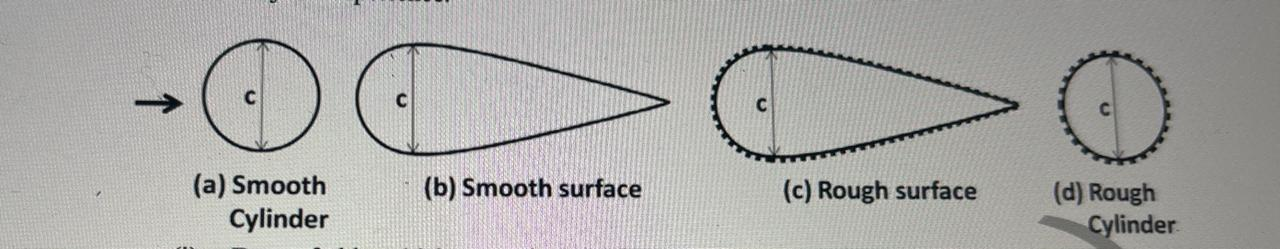
\includegraphics[width=0.5\columnwidth]{Figs/Q32.jpeg}
\caption{}
\end{figure}

\begin{enumerate}[label=(\roman*)]
    \item Drag of object (a) is more than the drag of object (d)  
    \item Drag of object (a) is less than the drag of object (d)  
    \item Drag of object (b) is more than the drag of object (c)  
    \item Drag of object (c) is more than the drag of object (b)  
    \item Drag of object (a) is more than the drag of object (b)  
\end{enumerate}

Choose the correct combination of statements from the options given above:  
\begin{enumerate}
    \item (i), (iii), (v)
    \item (ii), (iv), (v)
    \item (i), (iv), (v)
    \item (i), (iii)
\end{enumerate}
\hfill{\brak{\text{GATE AE 2014}}}


\item \quad A student needs to find velocity across a stationary normal shock. He measures density and pressure across the shock as shown in the figure below. (No shock table is needed for the calculations.) The value of $u_1$ in m/s is

\begin{center}
\begin{tabular}{c c c}
$P_1 = 1 \ \text{bar}$ & $\rho_1 = 1.2 \ \text{kg/m}^3$ & $\longrightarrow$ \\
& Shock & \\
$P_2 = 29 \ \text{bar}$ & $\rho_2 = 6 \ \text{kg/m}^3$ & $u_2$
\end{tabular}
\end{center}
\hfill{\brak{\text{GATE AE 2014}}}

\item \quad For inviscid, compressible flow past a thin airfoil, shown in the figure, free-stream Mach number and pressure are denoted by $M_\infty$ and $p_\infty$ respectively. Ratio of pressure at point A and $p_\infty$ is $0.8$ and specific heat ratio is $1.4$. If the Mach number at point A is $1.0$ and rest of the flow field is subsonic, the value of $M_\infty$ is:

\begin{figure}[H]
\centering
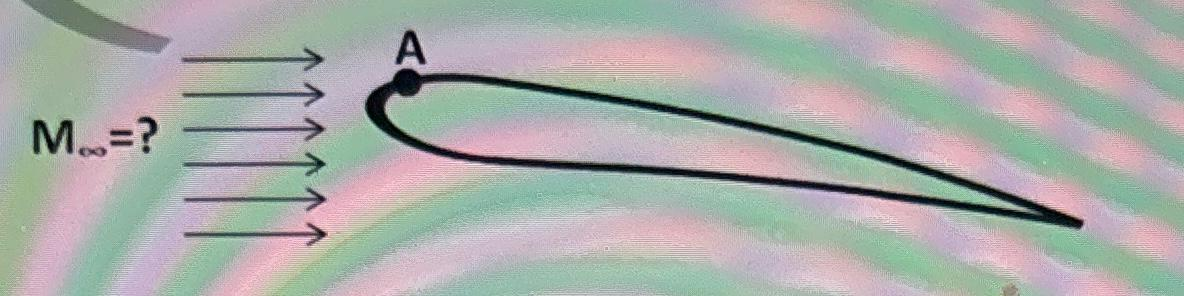
\includegraphics[width=0.5\columnwidth]{Figs/Q34.jpeg}
\caption{}
\end{figure}

\begin{multicols}{2}
\begin{enumerate}
    \item 2.95
    \item 0.79
    \item 1.18
    \item 0.64
\end{enumerate}
\end{multicols}
\hfill{\brak{\text{GATE AE 2014}}}

\item \quad A student can measure free-stream velocity of a low-speed wind tunnel using a:
\begin{enumerate}[label=(\roman*)]
    \item Pitot tube alone aligned with the flow direction.
    \item Pitot tube aligned with the flow direction with static pressure measurement at an appropriate position on the tunnel wall.
    \item Pitot tube aligned with the flow direction along with barometer pressure reading of the outside ambient.
    \item Pitot static tube alone aligned with the flow direction.
\end{enumerate}

Considering the above statements, which of the following options is correct?
\begin{multicols}{2}
\begin{enumerate}
    \item (i) only
    \item (i) \& (ii)
    \item (ii) \& (iv)
    \item (i), (iii) \& (iv)
\end{enumerate}
\end{multicols}
\hfill{\brak{\text{GATE AE 2014}}}

\item \quad Induced velocity $w$ at a point $z = z_1$ along the lifting line can be calculated using the formula  
$$
w(z_1) = -\frac{1}{4\pi} \int_{-S}^S \frac{d\Gamma/dz}{z_1 - z} \, dz
$$
Given  
$$
\frac{r^2}{T_0^2} + \frac{z^2}{S^2} = 1
$$ 
where $r, T_0$ and $S$ are given in the figure below.  

For the above semi-elliptic distribution of circulation,  
$$
\Gamma = \frac{\Gamma_0}{4\pi S} \int_{-S}^S \frac{\sqrt{S^2 - z^2}}{z_1 - z} \, dz
$$ 
the downwash velocity at any point $z_1$ for symmetric flight can be obtained as,  
$$
w(z_1) = \frac{\Gamma_0}{4\pi S} \left[ \pi r + z_1 I_1 \right], \quad I_1 = \int_{-S}^S \frac{\sqrt{S^2 - z^2}}{z_1 - z} \, dz
$$  

The induced drag is  
$$
D_i = \frac{\rho U_\infty}{S} \int_{-S}^S \sqrt{1 - \frac{z^2}{S^2}} \, dz = \frac{\pi S}{2}
$$ 

\begin{figure}[H]
\centering
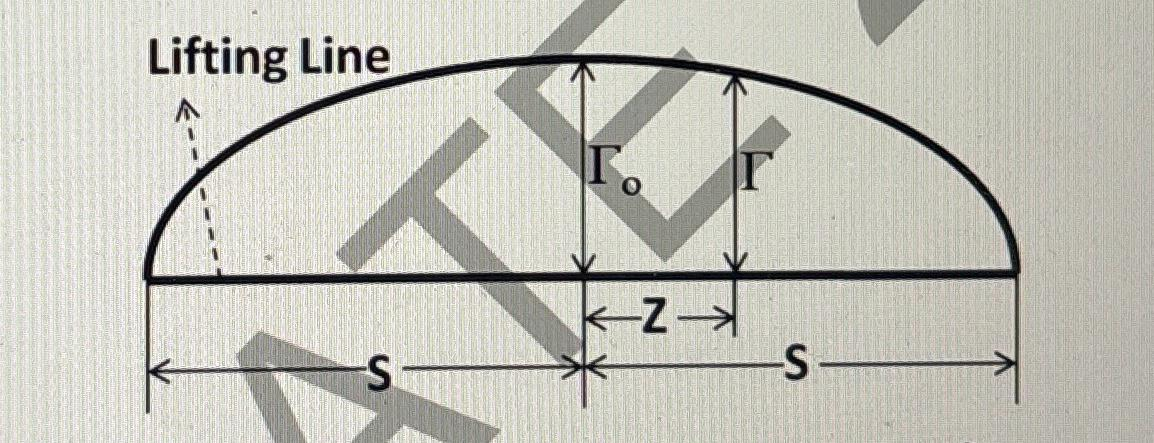
\includegraphics[width=0.8\columnwidth]{Figs/Q36.jpeg}
\caption{}
\end{figure}

Which of the following options is correct if the induced drag is $D_i$ (given $S$)?

\begin{multicols}{2}
\begin{enumerate}
    \item $l = 0$ and $D_i = \frac{8 \rho \Gamma_0^2}{\pi}$
    \item $l = l$ and $D_i = \frac{8 \rho \Gamma_0^2}{\pi}$
    \item $l = 0$ and $D_i = \frac{\pi \rho \Gamma_0^2}{8}$
    \item $l = l$ and $D_i = \frac{\pi \rho \Gamma_0^2}{8}$
\end{enumerate}
\end{multicols}

\hfill{\brak{\text{GATE AE 2014}}}

\item \quad Two overflowing water reservoirs are connected with a 100 m long pipe of circular cross-section (of radius $R = 0.02$ m), such that the height difference $h$ remains constant as shown in the figure below.  

The centerline velocity in the pipe is $10$ m/s. The velocity profile inside the pipe over the entire length is given as  
$$
u_z(r) = \frac{R^2}{4\mu} \frac{dp}{dx} \left[ 1 - \frac{r^2}{R^2} \right]
$$ 
where $\frac{dp}{dx}$ is a constant pressure gradient along the pipe length, $x$ is measured from the left end of the pipe along its central axis and $r$ is radial location inside the pipe with respect to its axis.  

Given: density and kinematic viscosity of water are $1000$ kg/m$^3$ and $1\times 10^{-6}$ m$^2$/s respectively, acceleration due to gravity is $10$ m/s$^2$.  

If all other losses except the frictional losses at the pipe wall are neglected, the value of $h$ in meters is:
\begin{figure}[H]
\centering
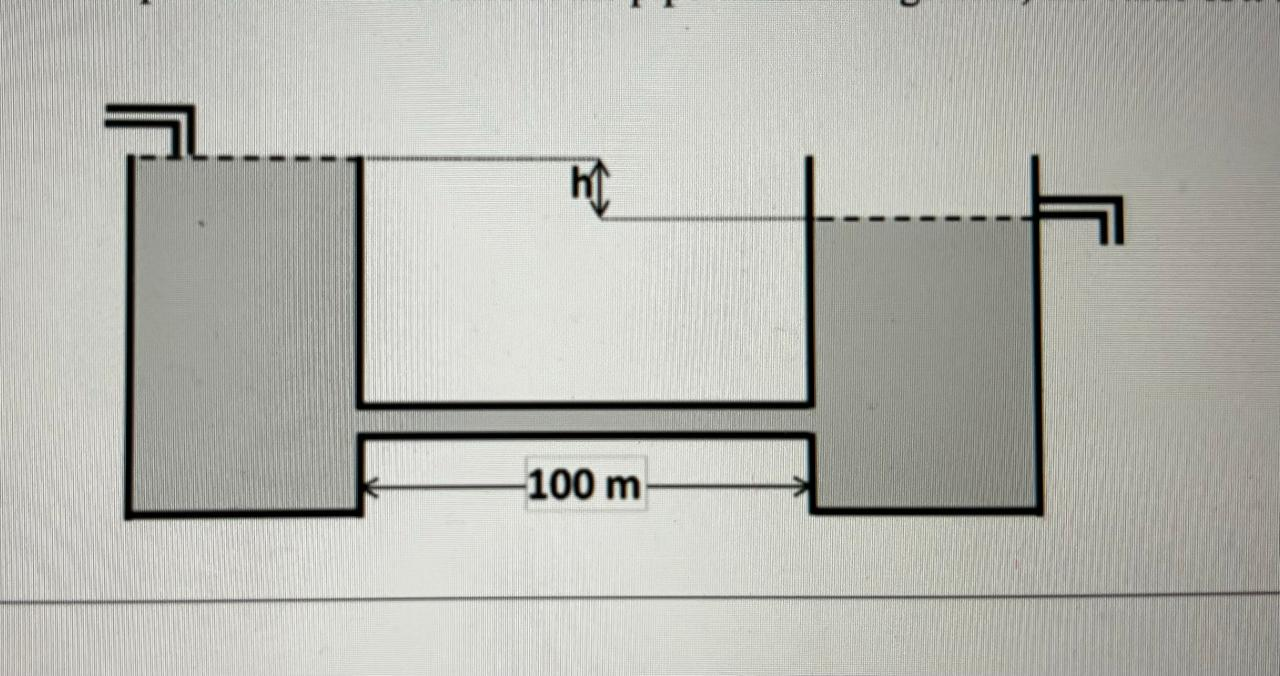
\includegraphics[width=0.5\columnwidth]{Figs/Q37.jpeg}
\caption{}
\end{figure}
\hfill{\brak{\text{GATE AE 2014}}}

\item \quad A 1.8 m long steel beam of rectangular cross section ($10 \text{ mm} \times 6 \text{ mm}$) is simply supported with a length of $1.2$ m between the supports and an overhang of $0.3$ m on either side. Young's modulus for the material of the beam is $200$ GPa. For a $50$ N load applied at the center of the beam, magnitude of the slope of the beam at tip S is:
\begin{figure}[H]
\centering
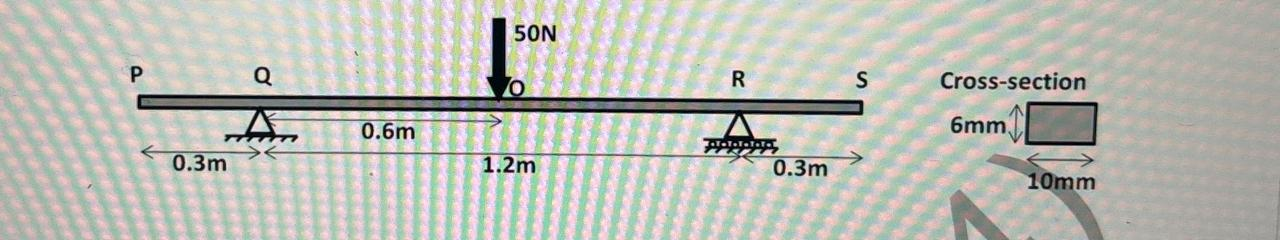
\includegraphics[width=0.5\columnwidth]{Figs/Q38.jpeg}
\caption{}
\end{figure}
\hfill{\brak{\text{GATE AE 2014}}}

\item \quad There are 2 designs proposed for a shaft of length $l$, with a torque carrying capacity of $T$. \textit{Design I} is a solid circular cross-section shaft of diameter $30$ mm. \textit{Design II} is a thin-walled circular shaft of average diameter $40$ mm. Thickness of the wall in \textit{Design II} has to be determined such that maximum shear stress is the same in both designs for the given torque $T$. The same material can be used for manufacturing both the shafts. Ratio of mass of shaft using \textit{Design I} to the mass of shaft using \textit{Design II} is:

\begin{figure}[H]
    \centering
    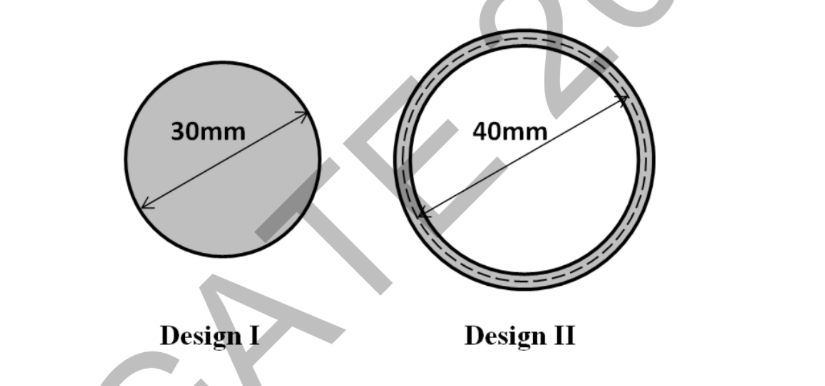
\includegraphics[width=0.5\columnwidth]{Figs/q49.png}
    \caption{Caption}
    \label{fig:placeholder}
\end{figure}

\begin{multicols}{2}
\begin{enumerate}
    \item 2.68
    \item 3.56
    \item 1.79
    \item 3.58
\end{enumerate}
\end{multicols}
\hfill{\brak{\text{GATE AE 2014}}}

\item \quad A structural member of rectangular cross-section ($10\ \mathrm{mm} \times 6\ \mathrm{mm}$) and length $1\ \mathrm{m}$ is made of steel (Young's modulus is $200\ \mathrm{GPa}$ and coefficient of thermal expansion is $12 \times 10^{-6} / ^\circ\mathrm{C}$). It is rigidly fixed at both the ends and then subjected to a gradual increase in temperature. Ignoring the three dimensional effects, the structural member will buckle if the temperature is increased by $\Delta T ^\circ\mathrm{C}$ which is:

\begin{figure}[H]
    \centering
    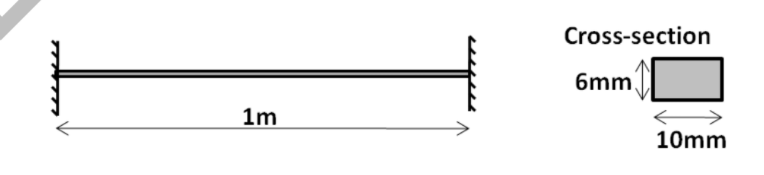
\includegraphics[width=0.5\columnwidth]{Figs/Q50.png}
    \caption{Caption}
    \label{fig:placeholder}
\end{figure}

\begin{multicols}{2}
\begin{enumerate}
    \item 19.74
    \item 9.87
    \item 78.96
    \item 39.48
\end{enumerate}
\end{multicols}
\hfill{\brak{\text{GATE AE 2014}}}

\item \quad A gas cylinder (closed thin-walled cylindrical pressure vessel) of diameter $30\ \mathrm{cm}$ and wall thickness $1\ \mathrm{mm}$ is subjected to a design maximum internal pressure of $5\ \mathrm{bar}$ ($0.5\ \mathrm{MPa}$). The material used for manufacturing this cylinder has a failure stress of $260\ \mathrm{MPa}$. Assuming von Mises failure criterion, the factor of safety (with respect to maximum allowable stress) for this cylinder is:

\begin{multicols}{2}
\begin{enumerate}
    \item 2.8
    \item 2.0
    \item 6.9
    \item 4.0
\end{enumerate}
\end{multicols}
\hfill{\brak{\text{GATE AE 2014}}}

\item \quad A cantilevered beam is subjected to a parabolic distribution of shear traction at the right edge while the top and bottom surfaces are traction free. To solve this problem, following Airy's stress function is proposed:  
$$
\phi = C_1 xy + C_2 x^3 y + C_3 x^2 y^2 + C_4 x y^3
$$  
This is an admissible Airys function that would satisfy the bi-harmonic equation as well as the boundary conditions if and only if

\
\begin{figure}[H]
\centering
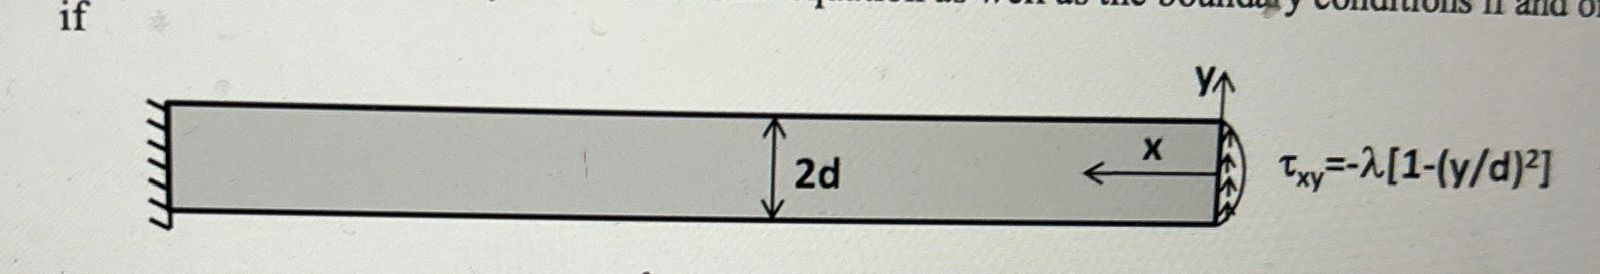
\includegraphics[width=0.4\columnwidth]{Figs/q42.jpeg}
\caption{}
\end{figure}


\begin{multicols}{2}
\begin{enumerate}
    \item $C_1 = 0,\ C_2 = \lambda,\ C_3 = 0,\ C_4 = \frac{\lambda}{3d^2}$
    \item $C_1 = \lambda,\ C_2 = \frac{\lambda}{3d^2},\ C_3 = 0,\ C_4 = 0$
    \item $C_1 = 0,\ C_2 = 0,\ C_3 = \lambda,\ C_4 = -\frac{\lambda}{3d^2}$
    \item $C_1 = \lambda,\ C_2 = -\frac{\lambda}{3d^2},\ C_3 = 0,\ C_4 = 0$
\end{enumerate}
\end{multicols}
\hfill{\brak{\text{GATE AE 2014}}}


\item \quad $1\ \mathrm{kg}$ mass is hanging from a spring of stiffness $500\ \mathrm{N/m}$ attached to a massless, symmetric beam of length $0.6\ \mathrm{m}$, moment of inertia about the bending axis $I = 8.33 \times 10^{-10}\ \mathrm{m}^4$ and Young's modulus $E = 210\ \mathrm{GPa}$ as shown in the figure. The fundamental natural frequency (in rad/s) of the system is:

\begin{figure}[H]
\centering
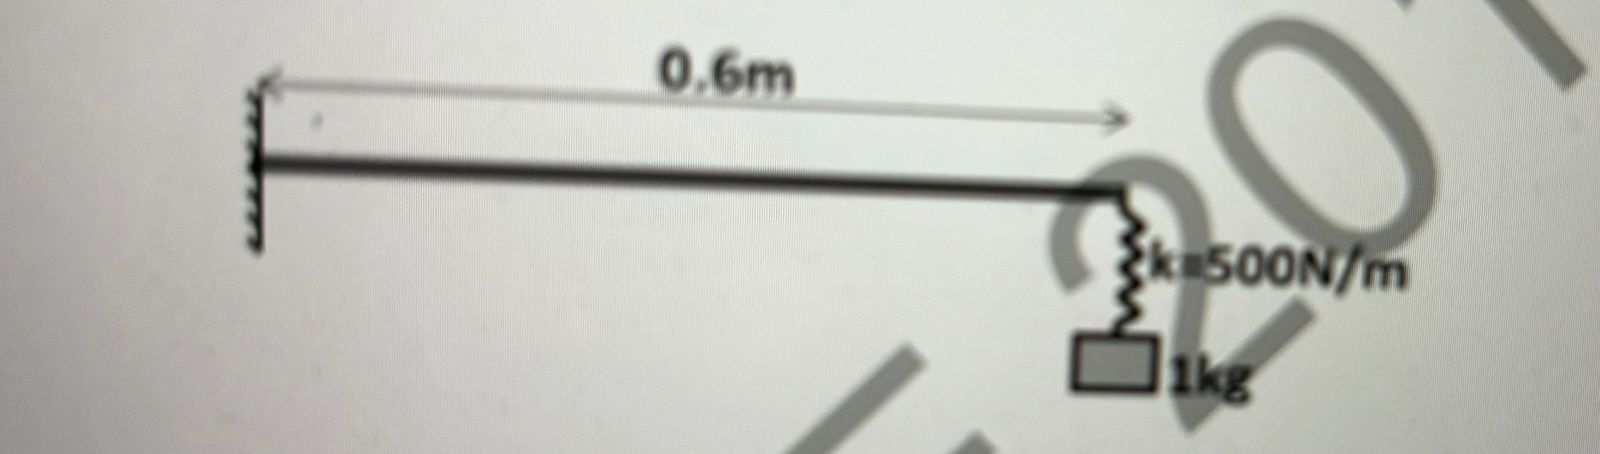
\includegraphics[width=0.5\columnwidth]{Figs/q43.jpeg}
\caption{}
\end{figure}

\begin{multicols}{2}
\begin{enumerate}
    \item 3.24
    \item 20.36
    \item 22.36
    \item 3.56
\end{enumerate}
\end{multicols}

\hfill{\brak{\text{GATE AE 2014}}}

\item \quad A single degree of freedom system is vibrating with initial (first cycle) amplitude of $5\ \mathrm{cm}$. The viscous damping factor associated with the vibrating system is $2\%$. Vibration amplitude of the fifth cycle (in cm) is:

\begin{multicols}{2}
\begin{enumerate}
    \item 1.65
    \item 4.41
    \item 2.67
    \item 3.02
\end{enumerate}
\end{multicols}
\hfill{\brak{\text{GATE AE 2014}}}

\item \quad A cruise missile with an \textit{ideal} ramjet engine is flying at Mach $4.0$ at an altitude where the ambient temperature is $100\ \mathrm{K}$. Considering specific heat ratio $\gamma = 1.4$ and specific gas constant $R = 287\ \mathrm{J/kg\cdot K}$. If the stagnation temperature in the combustion chamber is equal to $2310\ \mathrm{K}$, the speed of the exhaust gases (in m/s) is:

\hfill{\brak{\text{GATE AE 2014}}}

\item \quad  A gas turbine engine is operating under the following conditions: 
\begin{center}
\begin{tabular}{ll}
Stagnation temperature at turbine inlet & $1350 \ K$ \\
Stagnation pressure at the turbine inlet & $10 \ \text{bar}$ \\
Static temperature at turbine exit & $800 \ K$ \\
Velocity at turbine exit & $200 \ \text{m/s}$ \\
Total-to-total efficiency of turbine & $0.96$ \\
$\gamma$ (ratio of specific heats) & $1.33$ \\
$C_p$ (specific heat at constant pressure) & $1.147 \ \text{kJ/kgK}$ \\
\end{tabular} \\[6pt]
\end{center}
The stagnation pressure (in bar) in the nozzle (considering isentropic nozzle) is equal to \underline{\hspace{1.5cm}}.

 \hfill{\brak{\text{GATE AE 2014}}}
 
\item
Air at a stagnation temperature of $300 \ K$ (ratio of specific heats, $\gamma = 1.4$ and specific gas constant $R = 287 \ J/\text{kgK}$) enters the impeller of a centrifugal compressor in axial direction. The stagnation pressure ratio between the diffuser outlet and impeller inlet is $4.0$. The impeller blade radius is $0.3 \ m$ and it is rotating at $15000 \ \text{rev/min}$. If the slip factor $\sigma_s$ (Ratio of tangential component of air velocity at the blade tip to the blade tip speed) is $0.88$, the overall efficiency (total-to-total) of the compressor (in \%) is \underline{\hspace{1.5cm}}. 

\hfill{\brak{\text{GATE AE 2014}}}

\item 
A stationary two stage rocket with initial mass of $16000 \ \text{kg}$, carrying a payload of $1000 \ \text{kg}$, is fired in a vertical trajectory from the surface of the earth. Both the stages of the rocket have same specific impulse, $I_{sp}$, of $300 \ \text{s}$ and same structural coefficient of $0.14$. The acceleration due to gravity is $9.8 \ \text{m/s}^2$. Neglecting drag and gravity effects and considering both the stages with same payload ratio, the terminal velocity attained by the payload in m/s is \underline{\hspace{1.5cm}}. 

\hfill{\brak{\text{GATE AE 2014}}}

\item
An aircraft is flying at Mach $3.0$ at an altitude where the ambient pressure and temperature are $50 \ \text{kPa}$ and $200 \ K$ respectively. If the converging-diverging diffuser of the engine (considered isentropic with ratio of specific heats, $\gamma = 1.4$ and specific gas constant $R = 287 \ J/\text{kgK}$) has a throat area of $0.05 \ \text{m}^2$, the mass flow rate through the engine in $\text{kg/s}$ is  
\begin{enumerate}
    \item 197
    \item 232
    \item 790
    \item 157
\end{enumerate} 
\hfill{\brak{\text{GATE AE 2014}}}

\item 
A cryogenic rocket has a specific impulse of $455 \ \text{s}$ and characteristic velocity of $2386 \ \text{m/s}$. The value of thrust coefficient for this rocket is  
\begin{enumerate}
    \item 1.78
    \item 1.73
    \item 1.87
    \item 1.95
\end{enumerate} 
\hfill{\brak{\text{GATE AE 2014}}}

\item 
For a given airplane with a given wing loading executing a turn in the vertical plane, under what conditions will the turn radius be minimum and the turn rate be maximum?  
\begin{enumerate}
    \item Highest possible $C_L$ and lowest possible load factor  
    \item Lowest possible $C_L$ and lowest possible load factor  
    \item Lowest possible $C_L$ and highest possible load factor  
    \item Highest possible $C_L$ and highest possible load factor
\end{enumerate}
\hfill{\brak{\text{GATE AE 2014}}}

\item  
Lift-off distance for a given aircraft of weight $W$ is $S_{L0}$. If the take-off weight is reduced by $10\%$, then the magnitude of percentage change in the lift-off distance (assume all other parameters to remain constant) is \underline{\hspace{1.5cm}}. 
\hfill{\brak{\text{GATE AE 2014}}}

\item
Which of the following design parameters influence the maximum rate-of-climb for a jet-propelled airplane? 
P. Wing loading \\
Q. Maximum thrust-to-weight ratio \\
R. Zero-lift drag coefficient \\
S. Maximum lift-to-drag ratio \\[4pt]
\begin{enumerate}
    \item P and Q alone
    \item P, Q, R and S
    \item P, Q and S alone
    \item Q, R and S alone
\end{enumerate}
\hfill{\brak{\text{GATE AE 2014}}}

\item 
Consider the following four statements regarding aircraft longitudinal stability: \\[4pt]
P. $C_{M_{ac}}$ at zero lift must be positive \\
Q. $\frac{\partial C_{M_{ac}}}{\partial \alpha}$ must be negative ($\alpha$ is absolute angle of attack) \\
R. $C_{M_{ac}}$ at zero lift must be negative \\
S. Slope of $C_L$ versus $\alpha$ must be negative \\[4pt]
Which of the following combination is the necessary criterion for stick fixed longitudinal balance and static stability? \\[4pt]
\begin{enumerate}
    \item Q and R only
    \item Q, R and S only
    \item P and Q only
    \item Q and S only
\end{enumerate}
\hfill{\brak{\text{GATE AE 2014}}}

\item 
Data for a light, single-engine, propeller driven aircraft in steady level flight at sea-level is as follows: velocity $V_\infty = 40 \, \text{m/s}$, weight $W = 13000 \, \text{N}$, lift coefficient $C_L = 0.65$, drag coefficient $C_D = 0.025 + 0.04C_L^2$ and power available $P_a = 100{,}000 \, \text{W}$. The rate of climb possible for this aircraft under the given conditions (in m/s) is \underline{\hspace{1.5cm}}. \\[4pt]
\begin{enumerate}
    \item 7.20
    \item 5.11
    \item 6.32
    \item 4.23
\end{enumerate}
\hfill{\brak{\text{GATE AE 2014}}}
\end{enumerate}
\end{document}


